\section{Overview}
    L’espressione \textit{comunicazione dati} fa riferimento allo scambio (locale o remoto) di informazione fra due dispositivi attraverso un canale di comunicazione, il quale è caratterizzato da un mezzo trasmissivo (come un cavo). Affinché la comunicazione abbia luogo è necessario che i dispositivi siano parte di un sistema di comunicazione fatto di hardware e di software.

    \vspace{3mm}
    
    Un sistema di comunicazione è composto da \textit{messaggio} (i dati che devono essere inviati), \textit{mittente} (dispositivo che spedisce il messaggio), \textit{destinatario} (dispositivo che riceve il messaggio), \textit{mezzo trasmissivo} (cammino fisico sul quale il messaggio viaggia) e \textit{protocollo} (insieme di regole, adottate dai dispositivi) che governano la comunicazione).
    
    \vspace{3mm}
    
    Il \textbf{messaggio}, e cioè l'\textbf{informazione}, può essere rappresentata in varie forme, quali testi, numeri, immagini, audio, video e altro. Un messaggio è in \textit{forma discreta} se è rappresentato da sequenze di bit. Ad esempio, per il testo, la forma discreta coincide con una codifica ASCII; per le immagini, la forma discreta coincide con l'aggregazione di pixel.
    
    \vspace{3mm}
    
    La comunicazione fra due dispositivi può essere di tre tipi: \textbf{unidirezionale} (\textit{simplex}), \textbf{bidirezionale alternata} (\textit{duplex}) e \textbf{bidirezionale} (\textit{full-duplex}).
    
    \begin{itemize}
        \item 
        \textbf{Simplex:} La comunicazione avviene in una sola direzione, come succede al traffico automobilistico in una strada a senso unico. Solo uno dei due dispositivi può spedire dati mentre l’altro dispositivo può solo riceverli.
    
        \item
        \textbf{Duplex:} Ogni dispositivo può sia trasmettere che ricevere ma non contemporaneamente.
        
        \item
        \textbf{Full-Duplex:} Entrambi i dispositivi possono spedire e ricevere i dati contemporaneamente.
    \end{itemize}
    
    \subsection{Definizione di rete e connessione}
    
        Una \textbf{rete di calcolatori} (concettualmente nata col telegrafo nel 1840) è un insieme di dispositivi (detti \textit{nodi}) indipendenti ed interconnessi tra loro attraverso un canale di comunicazione, tramite il quale possono scambiarsi informazioni e cooperare. I vantaggi giacciono chiaramente nella possibilità di condividere risorse e collaborare, riducendo dunque i costi e distribuendo in modo omogeneo il peso computazionale. 
        
        Inoltre, una rete può garantire affidabilità e \textit{fault tolerance} (significa che, nell'eventualità del crash di un nodo, si ha a disposizione una copia replicata del servizio affinché l'utente comunque accedere al medesimo servizio). Lo svantaggio è che tutto ciò richiede una gestione difficoltosa e complessa.
        
        \vspace{3mm}
        
        Le connessioni che collegano i nodi di una rete possono essere classificate in due
        grandi categorie: \textit{connessioni punto-punto} e \textit{connessioni multipunto}.
        
        \begin{itemize}
            \item 
            Una \textbf{connessione punto-punto} si ottiene dedicando un canale fisico ai due dispositivi che devono comunicare. L’intera capacità del canale è dedicata ai due dispositivi connessi dal
            collegamento. Un esempio pratico è un cavo che connette due computer.
            
            \item
            Una \textbf{connessione multipunto} è un collegamento condiviso da più di due dispositivi. La capacità di un collegamento multipunto va condivisa fra i dispositivi che lo usano. La condivisione può avvenire temporalmente se l’accesso al mezzo trasmissivo è esclusivo, motivo per cui l'utilizzo del collegamento è \textit{a turnazione}. 
            
            Se il canale trasmissivo ammette un utilizzo simultaneo da parte di più dispositivi allora si parla di \textit{condivisione dello spazio}.
        \end{itemize}
        
        La \textbf{topologia} descrive come i nodi sono fisicamente connessi da un mezzo trasmissivo, e possono essere di quattro tipi: \textit{mesh}, \textit{stella}, \textit{bus} e \textit{anello}. E' anche possibile elaborare soluzioni ibride.
        
        \begin{itemize}
            \item 
            In una topologia \textbf{mesh} (\textit{a maglia di rete}), ogni nodo ha un collegamento punto-punto con ogni altro nodo della rete. 
            
            Utilizzando dei collegamenti simplex occorrono \(n*(n-1)\) collegamenti per una mesh; invece, utilizzando dei collegamenti duplex occorrerebbero \(n*(n-1)/2\) collegamenti.
            
            Il numero di collegamenti è quadratico rispetto al numero di nodi.
            
            Il vantaggio è che ogni coppia di nodi può comunicare indipendentemente da ogni altra coppia, assicurando affidabilità e sicurezza. Lo svantaggio è che serviranno molti cavi per collegare i nodi.
            
            \begin{center}
                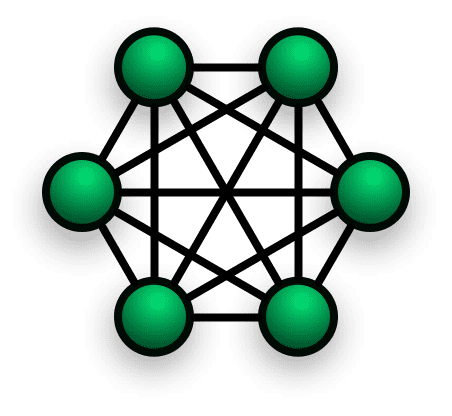
\includegraphics[scale=0.25]{images/MeshNetwork.png}
            \end{center}
            
            \item
            In una topologia a \textbf{stella}, ogni nodo è connesso con un collegamento punto-punto ad un dispositivo centrale chiamato \textbf{hub}. Tutto il traffico passa attraverso l'hub.
            
            E' una soluzione economica: se un nodo si rompe, non si compromette l'intera rete. Tuttavia, tutta la rete dipesa dall'hub, e se esso si rompe, l'intera rete diventa inutilizzabile.
            
            \begin{center}
                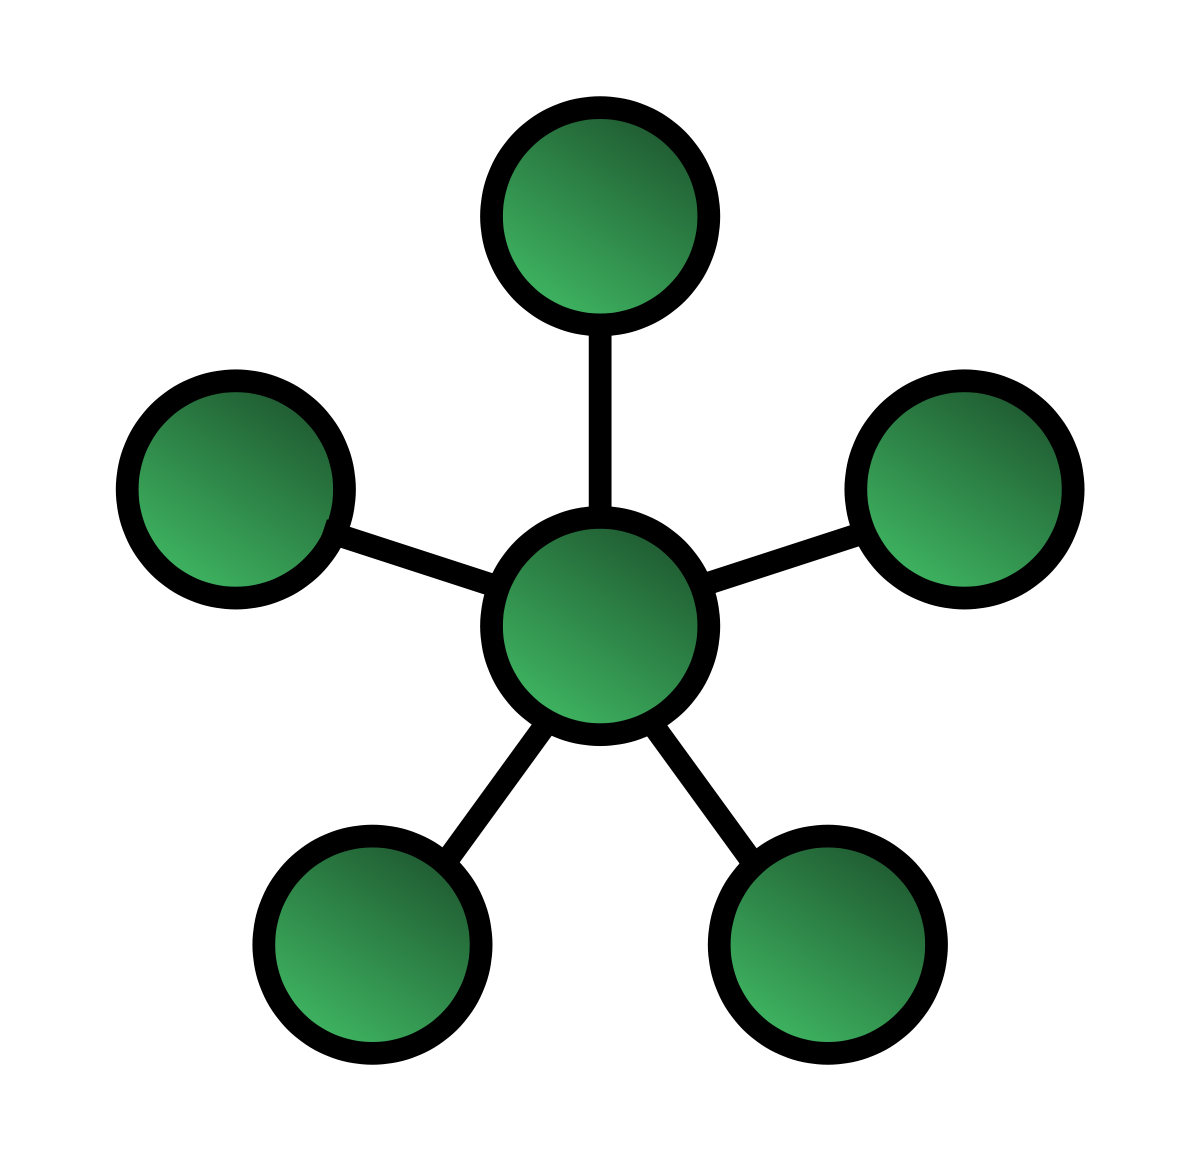
\includegraphics[scale=0.090]{images/StarNetwork.png}
            \end{center}
            
            \item
            In una topologia a \textbf{bus}, la rete utilizza un collegamento multipunto per connettere tutti i nodi. Ogni nodo è connesso al bus tramite un connettore fisico. Quando il segnale attraversa il bus, il connettore riesce a leggerlo.
            
            Il connettore è detto \textit{dorsale}.
            
            Un esempio di topologia con bus è l'Ethernet.
            
            Se il connettore è troppo lungo, il segnale perde d'intensità, limitando notevolmente il numero di connettori e quindi di nodi che si possono collegare al bus. Il vantaggio di questa soluzione è la facilità di installazione di un nuovo nodo. In ogni caso, la gestione dei problemi relativi al bus in sé è difficoltosa e un guasto al connettore potrebbe blocare tutte le connessioni.
            
            Inoltre, l'amministratore di rete deve posizionare adeguatamente i nodi affinché i connettori siano distanziati e non entrino in conflitto.
            
            \begin{center}
                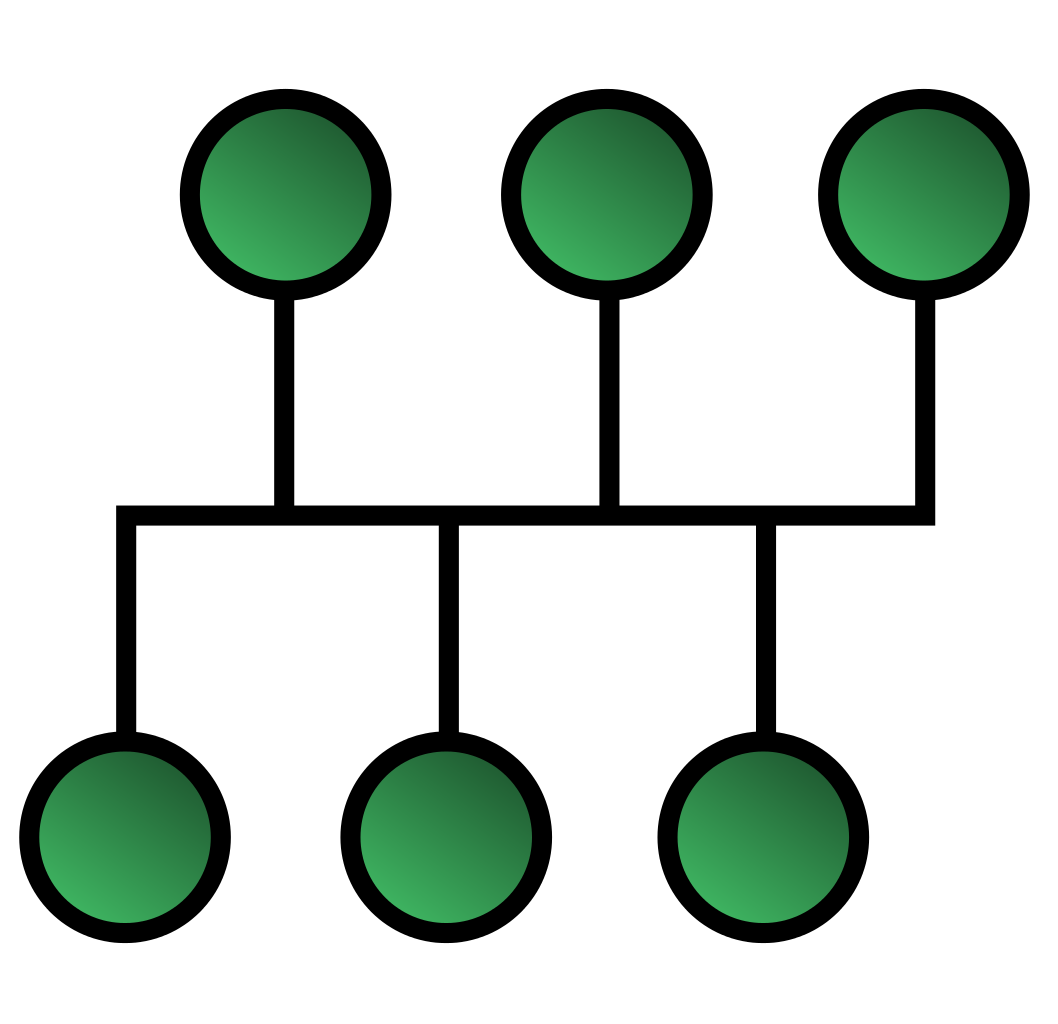
\includegraphics[scale=0.090]{images/BusNetwork.png}
            \end{center}
            
            \item
            In una topologia ad \textbf{anello}, ogni nodo ha un collegameno punto-punto con solo altri due nodi, cioè il nodo precedente e quello successivo. I dati viaggiano in una sola direzione, e ogni nodo ha un ripetitore che rigenera il segnale.
            
            Il vantaggio è che aggiungere un nodo o rimuoverlo richiede il cambiamento dei suoi due vicini e nient'altro; inoltre, isolare un guasto è molto semplice.
            
            Lo svantaggio è relativo alla natura unidirezionale del traffico. Se un ripetitore si rompe, l'intera rete diventa inutilizzabile. La soluzione al problema è l'aggiunta di un ulteriore anello, in modo tale da avere una comunicazione bidirezionale.
            
            \begin{center}
                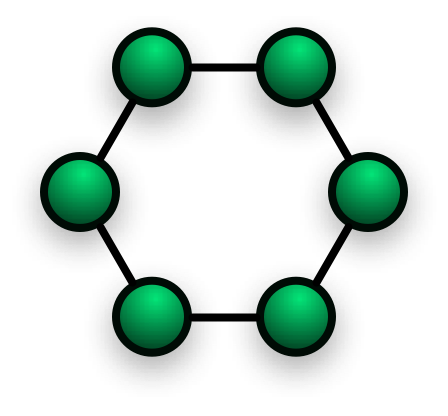
\includegraphics[scale=0.25]{images/RingNetwork.png}
            \end{center}
        \end{itemize}
        
        Le topologie ibride impiegano più tipi di topologie combinate.
    
    \subsection{Internet e Internet Service Providers}
    
        Una rete è categorizzabile anche in base alla sua dimensione (LAN, MAN, WAN, Interrete). Esistono molte "\textit{internet}", ma la più grande è "\textit{Internet}".
    
        \textbf{Internet} è una rete di reti che usa il protocollo TCP/IP (progenie del Dr. Vinton Cerf, citato per la prima volta nel 1974) e il \textit{Packet Switching} (i dati vengono impacchettati, suddivisi e seguono più percorsi per raggiungere la destinazione). 
        
        \vspace{3mm}
        
        La sua origine può essere datata al 1945 (grazie, fra gli altri, al pioniere Vannervar Bush, autore degli ipertesti - termine coniato in origine da Ted Nelson) e attribuita al progetto \textbf{Memex}, che si prefiggeva l'obiettivo di "\textit{mettere in relazione informazioni in maniera simile al cervello umano}", poi meglio concretizzato nella rete \textbf{ARPANET} degli Stati Uniti, il cui primo nodo è datato 1969 e che inizialmente connetteva fra i 4 e i 23 computer.
        
        Analogamente, Claude Shannon contribuì concenependo la rappresentazione binaria dei dati (\textbf{Modern Information Theory}), mentre Joseph Liklider concepì il computer come "\textit{communication device}"); Paul Baron inventò la commutazione di pacchetto, Vinton Cerf e Robert Kahn lavorarono al TCP/IP, Tim Barners-Lee introdusse l'HTTP e il WWW, e Mark Andreesen creò il primo web browser. Altre figure moderne importanti sono Steve Jobs, Paul Allen, Larry Page, Sergey Brin, Mark Zuckerberg, e molte altre.
        
        Dal 1994 al 1999, si susseguirono l'introduzione del World Wide Web, la nascita di Java, la pubblicazione di Windows 95 e la presentazione di VRML - tutti eventi che concorsero allo sviluppo di Internet, che ebbe il suo massimo splendore nella "guerra del commercio elettronico" fra Netscape e Microsoft del 1996-1997.
        
        \vspace{3mm}
        
        Uno sviluppo naturale di Internet è stato l'\textit{Internet of Things}, grazie al quale gli oggetti di tutti i giorni acquisiscono la capacità di comunicare e accedere ad informazioni aggregate.
        
        \vspace{3mm}
        
        I terminali accedono ad Internet attraverso gli \textbf{Internet Service Provider} (ISP), aziende istituzionali, aziendali o universitarie che forniscono accesso alla rete tramite sistemi wireless, DSL, dial-up, e così via. Gli utenti connessi con ISP diversi possono comunicare tra di loro perchè gli ISP a basso livello sono interconnessi ad ISP di livello più alto. Internet, infatti, funziona fondamentalmente tramite una gerarchia di ISP.
        
        \vspace{3mm}
        
        La struttura di Internet è organizzata a cerchi concentrici: si hanno ISP di livello 1 o "\textit{reti dorsali di Internet}" (AT\&T, Sprint, Telecom - è il livello più centrale dei cerchi concentrici), di livello 2 o "\textit{reti nazionali}", e di livello 3 o "\textit{reti locali}". Ciò significa che una richiesta passa attraverso più ISP, e quindi reti, per arrivare alla destinazione.
        
        Le reti dorsali di Internet sfruttano i "\textit{Core Routers}", cioè router efficienti e di grandi dimensioni situati in località strategiche.
    
    \subsubsection{Caratteristiche dei protocolli di rete}
    
        I sistemi terminali ed i commutatori di pacchetti fanno uso di \textbf{protocolli} (ossia regole che permettono la comunicazione fra due \textit{peer}) per l’invio e la ricezione dei dati. Un protocollo definisce il formato, l'interpretazione e l’ordine dei messaggi scambiati tra due o più entità in comunicazione, così come le azioni intraprese in fase di trasmissione e/o ricezione di un messaggio o di un altro evento.
        
        \vspace{3mm}
        
        Gli elementi chiave di un protocollo sono la \textbf{sintassi} (formato dei messaggi, ordine), la \textbf{semantica} (interpretazione dei bit) e la \textbf{sincronizzazione} (uniformità delle diverse velocità alla quale operano mittente e destinatario).
        
        \vspace{3mm}
        
        Una caratteristica comune dei protocolli di rete è il loro essere strutturati in \textbf{livelli sovrapposti}: il livello superiore esegue richieste al livello sottostante, e livelli uguali su macchine diverse conversano tramite lo stesso protocollo. Il vantaggio è che ogni strato non dipende strettamente dagli altri, e fornisce servizi comuni a tutte le funzioni dello strato superiore. 
        
        \vspace{3mm}
        
        Infine, gli \textit{standard} sono di fondamentale importanza per avere un mercato libero in cui i vari produttori di dispositivi possano operare per garantire l’interoperabilità di tali apparati. Forniscono delle linee guida a chiunque (produttori di hardware e software, venditori, agenzie governative, fornitori di servizi) sia coinvolto nello sviluppo di una interrete pubblica. Si classificano in "\textit{de facto}" e "\textit{de jure}". 
        
        Chiaramente, anche Internet segue degli standard. La proposta per l'introduzione di un nuovo standard è chiamata "\textit{draft}"; se la proposta viene approvata, diventa un RFC (\textit{Request For Comment}). Valutata la fattibilità e maturata la proposta, essa diventa uno standard universalmente accettato.
